\documentclass[11pt]{article}

\title{Using SAS on Mathlab}
\author{}
\date{}

\usepackage{graphicx}

\begin{document}
\maketitle

\section{Introduction}
\label{sec:intro}

This is not a mathematical course, but it does involve
computing. Specifically, we will be using the statistical package SAS:
learning how to analyze data using the methods we learn, and how to
interpret the output.

SAS has been around for years (now on version 9), and has become the
standard in industry, government and suchlike places for ``routine''
statistical analysis (that is, where more or less well-known
statistical procedures are to be used). If you can say, therefore,
that you have experience with SAS, it makes you that much more
employable! SAS runs on Windows, Unix, the Mac, etc; it is big, and
expensive, but there are certain common themes, and, as we will see,
once you see how to run one analysis, you can easily learn how to run
another. SAS is not point-and-click: you write a ``program'' and then
run it, but you then have the advantage of knowing exactly what you
did, and being able to run the program again, or modify it. Is SAS
user-friendly? No. And certainly not the way we use it.
But the input and output from SAS look exactly the same in
every environment: Windows, Unix, running on your machine or some
remote machine. So what you learn here will definitely be transferrable to
what you might see later.

SAS can be run in two ways. One is a ``batch mode'', where you submit
commands, get some output, look to see whether the output is what you
expected, and if not, try again. There is also a ``development
environment'' where you get a rather counter-intuitive editor that you
can use to construct your commands with.  We're going to stick with
the batch mode, because you can use a much more intuitive editor to
construct things with.

At UTSC, SAS runs on a Linux machine called Mathlab, on which you have
(or will have) an account. Thus, the first step is to get things set
up on Mathlab.

\section{Setup}

You will need a \emph{username} and \emph{password}. These are your
UTSC ID and password, the ones you use for accessing your UTSC e-mail
(if you do that) or the Intranet (unless you use your UTorID for
that). If you're enrolled in STAD29, this should be ready to go; if
you're in STA 1007, I might have to help you out. Test it and see
whether it works.

If you happen to be running Linux (or a Mac), 
there's no other setup required, beyond being able to open a terminal
(command-line) window. 

In the likelier event that you're running Windows, you have a couple
of things to organize first. 

First you need a program called \verb-Xming- that allows SAS's
windowing environment to happen in Windows (even though Mathlab runs
Ubuntu Linux). Download this from
\verb-sourceforge.net/projects/xming-, clicking on the big green
button, and install it in the usual way. Allow it to place a shortcut
on your desktop for ease of use later.

Then you need a program called \verb-putty-, which you can get from
\verb-putty.org-. This actually enables you to connect to
Mathlab. Just download \verb-putty.exe- and save it on your desktop
--- there's no install required. (Choose ``save'' rather than ``run''
to download it.)

To test your installation, first run Xming by double-clicking on its
icon. This will appear to do nothing except put a big X in your system
tray. Now start Putty as well (ignoring any ``unknown publisher''
warnings). There are a few things to enter before you can connect to
Mathlab. In the Host name box, enter
\verb-mathlab.utsc.utoronto.ca-. Leave Port 22 and Connection Type SSH
as they are. Then in the Category window on the left, look for SSH
with a plus sign next to it (down near the bottom). Click on the plus
sign. Look for X11 in the choices that pop out (the fourth one). Click
on it. On the right there is ``Enable X11 forwarding'' with a check
box next to it. Click on the check box. Then look in the Category
window on the left for Session (right at the top) and click on
it. This takes you back to where you started. Save this (so you don't
have to do it every time) by first typing a name like \verb-mathlab-
into the Saved Sessions box, and then clicking on the Save button on
the right. The name you chose appears in the bottom box below Default
Settings.

Now you can get connected. In Putty, click Open. This will bring up a
black screen asking for your Mathlab username and password (the same
as your UTSCid ones). If you can't log in, check your password, and if
you still can't, let me know. If you can, you'll see some stuff
including ``Ubuntu comes with ABSOLUTELY NO WARRANTY'', and then it
waits for you to type something. We'll see in a moment what you might
type. 

\section{Connecting to Mathlab}
\label{sec:runsas}

On Linux or a Mac,
open up a terminal window and type

\begin{verbatim}
ssh -X username@mathlab.utsc.utoronto.ca
\end{verbatim}

where you replace \verb-username- with your actual UTSC
username. Jump over the next paragraph, and ignore anything about Xming.

On Windows, start up Xming, then run Putty, loading your saved
\verb-mathlab- profile (click on \verb-mathlab-, then click
Load). Click Open to connect. Enter your username (UTSCid) when
prompted.

Then enter your password (the one that goes with your UTSCid). If it
doesn't work, check it and try again; if it still doesn't work, ask
me.

You'll see a whole bunch of things indicating that you are connected
to Mathlab. 


\section{Using SAS}
\label{UsingSAS}

To begin with, we'll need a text editor. This will be used for
entering our SAS commands, and also for looking at the output. The
text editor we'll use on Mathlab is called \texttt{kwrite}; it looks
and works much like Notepad on Windows.

The way SAS works is that you write out a bunch of commands to tell
SAS what you'd like it to do, run SAS on those commands, and then
(with luck) you get some output to look at. Think of a name for your
first SAS file, like \texttt{first.sas}, and then open it up in
\texttt{kwrite} by typing \texttt{kwrite~first.sas~\&}. The ampersand
on the end is important; if you forget it, you won't be able to do
anything else until you close the editor window.

Into \texttt{first.sas} (or whatever you called it), type the
following lines. You need to make sure that every line ends with a
\texttt{;} except for the lines consisting only of numbers:

\filbreak
\begin{verbatim}
data mydata;
  input x;
  cards;
1
2
3
5
7
;

proc print;

proc means;

run;
\end{verbatim}
\filbreak

This means the following:

\begin{itemize}
\item Here comes a data set called \verb-mydata-, with one variable,
  called \verb-x-. 
\item Here come the data values. (You can use \verb-datalines- instead
  of \verb-cards-, but I like the throwback to the days of punched cards.)
\item The five values for \verb-x- are 1,2,3,5 and 7.
\item \verb-proc print- just lists the data, so you can check that the
  values were read in properly.
\item \verb-proc means- calculates means and SDs for all the variables
  (just \verb-x-, here).
\end{itemize}

Once you have this right to your satisfaction, see whether it
works. Save the file,
go back to the terminal (Putty) window, press Enter if you need to,
then type \texttt{sas first.sas} followed by Enter. You won't see any
output, or even 
any indication that anything worked, or not. Don't worry about that. 

First we see whether it worked. Go back to your \texttt{kwrite} window
and open the file \texttt{first.log}. Mine looks like this, after some
preamble: 

\filbreak
\begin{verbatim}
NOTE: SAS initialization used:
      real time           0.09 seconds
      cpu time            0.04 seconds
      
1          data mydata;
2            input x;
3            cards;

NOTE: The data set WORK.MYDATA has 5 observations and 1 variables.
NOTE: DATA statement used (Total process time):
      real time           0.01 seconds
      cpu time            0.01 seconds
      
9          ;
10         
11         proc print;
12         

NOTE: There were 5 observations read from the data set WORK.MYDATA.
NOTE: The PROCEDURE PRINT printed page 1.
NOTE: PROCEDURE PRINT used (Total process time):
      real time           0.21 seconds
      cpu time            0.09 seconds
      

13         proc means;
14         
15         
NOTE: There were 5 observations read from the data set WORK.MYDATA.

2                                                          The SAS System                            21:35 Monday, December 26, 2011

NOTE: The PROCEDURE MEANS printed page 2.
NOTE: PROCEDURE MEANS used (Total process time):
      real time           0.05 seconds
      cpu time            0.03 seconds
      

NOTE: SAS Institute Inc., SAS Campus Drive, Cary, NC USA 27513-2414
NOTE: The SAS System used:
      real time           0.37 seconds
      cpu time            0.18 seconds

\end{verbatim}

All being well, you'll get a collection of \texttt{NOTE}s telling you
what data were read in, which procedures were run on the data, and how
much time it all took. (It's a good idea to make sure you got as much
data as you expected; here 5 observations on one variable is correct.)

Suppose I mistakenly typed \verb-proc means- as
\verb-proc meanbubbles-. I'd get just the output
from \verb-proc print- in my output file and this in my log file:

\filbreak
\begin{verbatim}
1    data x;
2      input x;
3      cards;

NOTE: The data set WORK.X has 5 observations and 1 variables.
NOTE: DATA statement used (Total process time):
      real time           0.46 seconds
      cpu time            0.01 seconds

9    ;
10
11   proc print;
12

NOTE: There were 5 observations read from the data set WORK.X.
NOTE: PROCEDURE PRINT used (Total process time):
      real time           0.20 seconds
      cpu time            0.05 seconds


13   proc meanbubbles;
ERROR: Procedure MEANBUBBLES not found.
14
15   run;

NOTE: The SAS System stopped processing this step because of errors.
NOTE: PROCEDURE MEANBUBBLES used (Total process time):
      real time           0.05 seconds
      cpu time            0.00 seconds

\end{verbatim}
\filbreak

This all means:

\begin{itemize}
\item The data were read in properly.
\item \verb-proc print- worked just fine (no errors) and any output
  from it will appear in the Output window.
\item \verb-proc meanbubbles- does not exist, so SAS can't run
  it. This is (predictably) an Error.
\end{itemize}

SAS isn't always very forthcoming about what an error actually is, but
looking at the log file will at least tell you where in the file the
problem is (line 13 in my case). If you have an error, go back to the
\texttt{first.sas} file and fix it up. Save the file again. Then close
up \texttt{first.log} and go back to the terminal window. There, type
\texttt{sas first.sas} again and make sure \texttt{first.log} has no
errors this time. 

Once you are error-free, you can have a look at the output. This lives
in the file \texttt{first.lst}. Go back to \texttt{kwrite} and open
this up. You'll see:

\filbreak
{\footnotesize
\begin{verbatim}
                                           The SAS System         09:57 Monday, January 10, 2011   2

                                              Obs    x

                                               1     1
                                               2     2
                                               3     3
                                               4     5
                                               5     7
\end{verbatim}
}
\filbreak

which is the output of \verb-proc print-, and on the next page:

\filbreak
{\footnotesize
\begin{verbatim}
                                           The SAS System         09:57 Monday, January 10, 2011   3

                                        The MEANS Procedure

                                       Analysis Variable : x

                 N            Mean         Std Dev         Minimum         Maximum
                 -----------------------------------------------------------------
                 5       3.6000000       2.4083189       1.0000000       7.0000000
                 -----------------------------------------------------------------
\end{verbatim}
}
\filbreak

\verb-proc print- confirms that the data were read in correctly, while
\verb-proc means- actually tells us something interesting about the data.

The output is rather wide (actually 132 columns wide) and needed to be
shrunk considerably to get it on the page. This goes back to the days
of the big old line printers (with their enormous sheets of
tractor-feed paper), which were that wide. 80 columns is a better
width these days. To produce that, put the following line at the
\emph{top} of \texttt{first.sas} (and every other SAS file you want to
use it in):

\begin{verbatim}
options linesize=80;
\end{verbatim}

with this output:

\filbreak
{\small
\begin{verbatim}
                                 The SAS System                                5
                                                  09:57 Monday, January 10, 2011

                              The MEANS Procedure

                             Analysis Variable : x

       N            Mean         Std Dev         Minimum         Maximum
       -----------------------------------------------------------------
       5       3.6000000       2.4083189       1.0000000       7.0000000
       -----------------------------------------------------------------
\end{verbatim}
}
\filbreak

which required a good bit less shrinking to get it onto the page.

\section{How to get data from another file}

Rather than embedding your data into your programming code, you can
also save your data into a file. One way to do this is to type your
data into \texttt{kwrite} and then save it into a file on
Mathlab, traditionally with the extension \verb-.dat-. The data layout
(unless you are prepared to go through some contortions in SAS) is one
observation per line, with values for all the variables separated by
whitespace. The data below are values of a response variable $y$ from
three groups labelled a, b, and c:

\filbreak
\begin{verbatim}
a 20
a 21
a 16
b 11
b 14
b 17
b 15
c 13
c 9
c 12
c 13
\end{verbatim}
\filbreak

You can type these, into a new file in \texttt{kwrite}, then save it
as \verb-threegroups.dat-. Then you can create another file in
\texttt{kwrite} called \texttt{threegroups.sas}
and type the following program:

\filbreak
\begin{verbatim}
options linesize=80;

data groups;
  infile 'threegroups.dat';
  input group $ y;

proc print;

proc means;
  class group;
  var y;

run;
\end{verbatim}
\filbreak

Note that the filename has {\em single} quotes around it. This a bit
cleaner than the code with \verb-cards- (or \verb-datalines-) and the
actual data in it, because you can see rather more clearly what's
going on. Running this produces no errors (check the Log window to be
sure) and two pages of output. The first just lists the data, like
this:

\filbreak
{\small
\begin{verbatim}
                                 The SAS System                                6
                                                  09:57 Monday, January 10, 2011

                               Obs    group     y

                                 1      a      20
                                 2      a      21
                                 3      a      16
                                 4      b      11
                                 5      b      14
                                 6      b      17
                                 7      b      15
                                 8      c      13
                                 9      c       9
                                10      c      12
                                11      c      13
\end{verbatim}
}
\filbreak

and the second shows the means for each group separately:

\filbreak
{\small
\begin{verbatim}
                                 The SAS System                                7
                                                  09:57 Monday, January 10, 2011

                              The MEANS Procedure

                            Analysis Variable : y

             N
group      Obs    N           Mean        Std Dev        Minimum        Maximum
-------------------------------------------------------------------------------
a            3    3     19.0000000      2.6457513     16.0000000     21.0000000

b            4    4     14.2500000      2.5000000     11.0000000     17.0000000

c            4    4     11.7500000      1.8929694      9.0000000     13.0000000
-------------------------------------------------------------------------------

\end{verbatim}
}
\filbreak

As you would guess from looking at the data, group A has the largest
mean and group C the smallest.

%%%%%%%% this still needs fixing
%%%%%%%% also include stuff about plots

\section{Plots}
\label{sec:plots}

%%% use regression data with plot and gplot

Plots are not SAS's strength (not a huge surprise considering that SAS
dates from long before laser printers and graphics terminals). There
are two ways you might get a plot out of SAS, as shown below. These
are a proper graphics plot (in its own window), and a character-based
plot (which comes with the rest of the output). The graphics plot is
nicer if you can make it work, but sometimes the character-based plot
does the job just as well, and is easier to deal with.

Let's have a look at two different ways to get a scatterplot.

\begin{verbatim}
options ls=80 ps=50;

data xy;
  input x y;
  cards;
1 5 
2 6
3 4
4 8
5 11
;

proc gplot;
  plot y*x;

proc plot;
  plot y*x;

proc reg;
  model y=x;

\end{verbatim}

The options at the top sets the line width to be 80 columns
(\texttt{ls} is an abbreviation for \texttt{linesize}) and also the
number of \emph{rows} on a page to be 50 (\texttt{ps} is
\texttt{pagesize}). Then some $x$-$y$  data with $y$ going (more or
less) up as $x$ does. 

The \texttt{proc gplot} produces a graphics plot of $y$ vs $x$ in its
own window. The \texttt{proc plot} produces an old-fashioned
character-based plot in with the rest of the output. To make sure
there \emph{is} some other output to put the plot with, I've run a
regression to predict $y$ from $x$; this should have a positive slope,
since the trend appears to be uphill.

Running SAS gives you a graphics window with the scatterplot in it,
like this:

\filbreak
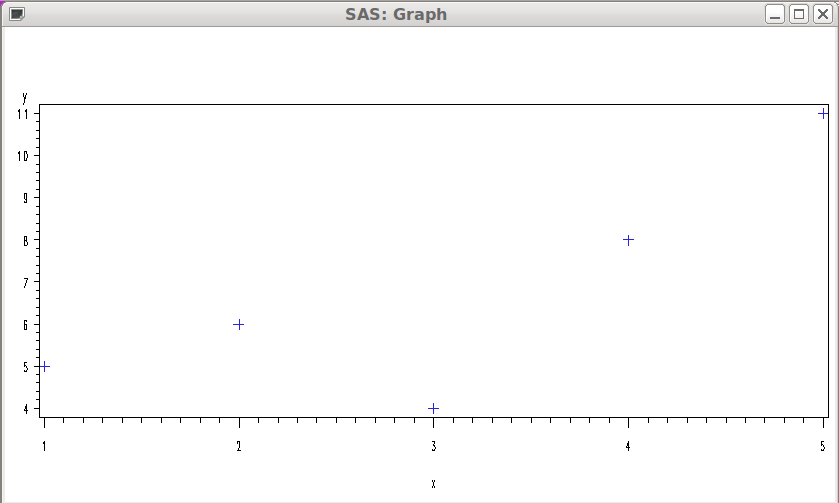
\includegraphics[width=4in]{plot1}
\filbreak

Mathlab will wait until you close this window; we'll talk below about
copying and pasting graphs, so for now you can note that the trend is
more or less uphill, then just close it and see
what other output you have in your \texttt{plot.lst} file.

There are two pages of it. First is the character version of the above
graph:

\filbreak
{\footnotesize
\begin{verbatim}
                Plot of y*x.  Legend: A = 1 obs, B = 2 obs, etc.

      y |
        |
     11 +                                                              A
        |
        |
        |
        |
     10 +
        |
        |
        |
        |
      9 +
        |
        |
        |
        |
      8 +                                               A
        |
        |
        |
        |
      7 +
        |
        |
        |
        |
      6 +                 A
        |
        |
        |
        |
      5 +  A
        |
        |
        |
        |
      4 +                                A
        |
        ---+--------------+--------------+--------------+--------------+--
           1              2              3              4              5

                                         x
\end{verbatim}
}
\filbreak

This tells the same story as the graphics plot, but a little more
crudely. If you are plotting a lot of points, some of them might need
to appear in the same place on the page; SAS distinguishes these by
plotting single points with an A, two points that landed up in the
same place with a B, and so on. Thus, if you see a D on a character
plot, \emph{four} points had to be plotted in the same place, either
because there were four identical data values or because they were
very close.

The second page of the output comes from the regression:

\filbreak

{\footnotesize
\begin{verbatim}
                               The REG Procedure
                                 Model: MODEL1
                             Dependent Variable: y 

                    Number of Observations Read           5
                    Number of Observations Used           5


                              Analysis of Variance
 
                                     Sum of           Mean
 Source                   DF        Squares         Square    F Value    Pr > F

 Model                     1       19.60000       19.60000       5.25    0.1058
 Error                     3       11.20000        3.73333                     
 Corrected Total           4       30.80000                                    


              Root MSE              1.93218    R-Square     0.6364
              Dependent Mean        6.80000    Adj R-Sq     0.5152
              Coeff Var            28.41446                       


                              Parameter Estimates
 
                           Parameter       Standard
      Variable     DF       Estimate          Error    t Value    Pr > |t|

      Intercept     1        2.60000        2.02649       1.28      0.2896
      x             1        1.40000        0.61101       2.29      0.1058
\end{verbatim}
}

\filbreak

The slope, at 1.4, is indeed positive, but it is not
\emph{significantly} different from zero; the P-value for that test is
smallish (0.1058) but not as small as the usual cutoff 0.05 for
significance. You might have guessed this from the plot; the upward
trend is not \emph{completely} convincing, and we do after all only
have 5 observations. R-squared for the regression is 0.64 (which means
that the correlation between $x$ and $y$ is about 0.8); this is quite
high, but still the kind of thing that can happen by chance with
$n=5$, even if there is no relationship in actuality.

\section{Copying and pasting}
\label{sec:copypaste}

Input to and output from SAS is plain text (except for the
``graphics'' graphs), and \texttt{kwrite} has an Edit menu that works
as you would expect. (This includes control-C and control-V, if you
use those keys.) This means that you can copy your code, output etc.\
into Word, or whatever you use, directly from \texttt{kwrite}. Keep in
mind that SAS uses a fixed-width font, so to keep those tables lined
up and to keep those character graphs looking as they should, you'll
need to use a fixed-width font like Courier or Lucida Console
yourself. Use a small enough font so that lines don't get wrapped. A
proportional font with wrapping lines looks \emph{really} ugly!

Graphics graphs are another matter. The best solution I've been able
to find is to take a screenshot of your graph window by clicking on
it, then pressing Alt-PrintScreen. This copies whatever you've taken a
screenshot of to the clipboard, from where you should be able to paste
it into your document. (I've tested this with WordPad, and it works
for me; last year's students had some trouble doing this with
Word. You shouldn't need anything more than WordPad for your
assignments if you want to use that.)

Copying and pasting \emph{into} SAS depends on whether you are copying
data values from a text editor like Notepad, from a web page, or from
a spreadsheet. In the first two cases, everything should work
properly, but in the third, the values can get copied with tabs in
between them.

For example, suppose your spreadsheet contains this:

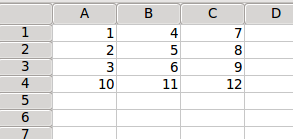
\includegraphics[width=3in]{s-data}

You can copy the values into \texttt{kwrite} and save them as a file, say
\verb-x.dat-, but then you need to read them into SAS like this:

\filbreak
\begin{verbatim}
data x;
  infile 'x.dat' delimiter='09'x;
  input a b c;

proc print;

run;
\end{verbatim}
\filbreak

where the gobbledegook after \verb-delimiter- means (to SAS) that the
data values are separated by tabs, and you correctly get this output:

\filbreak
{\small
\begin{verbatim}

                                 The SAS System                               10
                                                  09:57 Monday, January 10, 2011

                             Obs     a     b     c

                              1      1     4     7
                              2      2     5     8
                              3      3     6     9
                              4     10    11    12
\end{verbatim}
}
\filbreak

If you don't put in the \verb-delimiter- part, you will get a large
number of incomprehensible error messages.


\end{document}
